\documentclass[a4paper, 12pt]{article}
\usepackage[top=3cm, bottom=2cm, left=2cm, right=3cm]{geometry}
\usepackage[utf8]{inputenc}
\usepackage{amsmath, amsfonts, amssymb}
\usepackage{graphicx, xcolor}
\usepackage{tikz}
\usepackage{subfig}
\usetikzlibrary{arrows.meta}
\usetikzlibrary{calc}
\usepackage{scalerel, pict2e, tkz-euclide}
\usetikzlibrary{calc, patterns, arrows.meta,shadows,external}

\usepackage{pgfplots}
\usepackage{cancel}
\usepackage{enumitem}
\pgfplotsset{compat=newest}
\usepgfplotslibrary{statistics,fillbetween}
\usepackage{indentfirst}
\usepackage{babel}[pt-br]

\begin{document}
	\begin{figure}[ht]
		\centering
		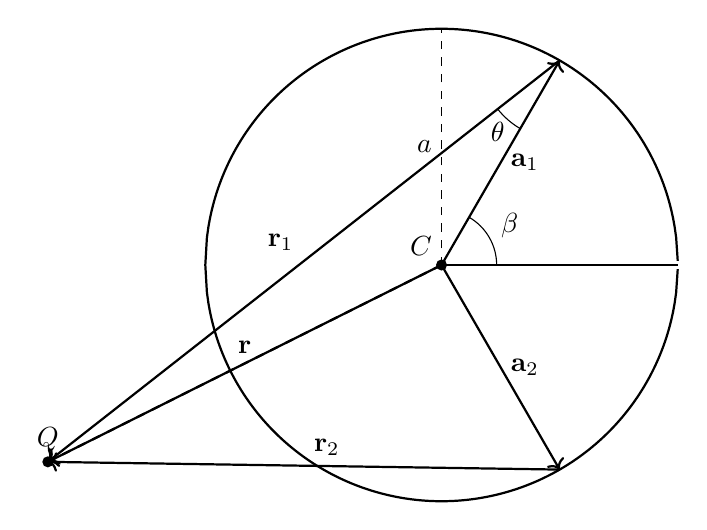
\begin{tikzpicture}
			
			
			\coordinate (A) at (0,0);
			\coordinate (B) at (-5,-2.5);
			\coordinate (C) at (1.5,2.598076211);
			\coordinate (D) at (1.5,-2.598076211);
			\coordinate (E) at (3,0);
	
			
			\draw[thick, domain=-3:3, samples=300] plot(\x, {sqrt(9-pow(\x,2))});
			\draw[thick, domain=-3:3, samples=300] plot(\x, {-sqrt(9-pow(\x,2))});
			
			\draw[thick,dashed, domain=-5:0, samples=300] plot(\x,{0.5*\x});
			\draw[dashed] (A) -- (0,3) node[midway,left]{$a$};
			\draw[->, thick] (C) -- (B) node[midway,above left]{$\textbf{r}_1$};
			\draw[->, thick] (D) -- (B) node[midway, above right]{$\textbf{r}_2$};
			\draw[->,thick] (A)--(B) node[midway, above]{$\textbf{r}$};
			
			\draw[->, thick] (A)--(C) node[midway, right] {$\textbf{a}_1$};
			
			\draw[->, thick] (A)--(D) node[midway, right] {$\textbf{a}_2$};
			
			\draw (A)--(E) ;
			
			\fill (A) circle (2pt) node[above left]{$C$};
			\fill (B) circle (2pt) node[above]{$Q$};
			
			\tkzMarkAngle(B,C,A);
			\tkzLabelAngle[pos=1.2](B,C,A){$\theta$};
			
			\tkzMarkAngle[size=0.7](E,A,C);
			\tkzLabelAngle[pos=1](E,A,C){$\beta$};
			
			
		\end{tikzpicture}
	\end{figure}
	
	A força $d\textbf{F}_1$ é então:
	
	\[
	d\textbf{F}_1=k\frac{Qdq}{r^3}\textbf{r}_1
	\]
	
	Escrevendo $\textbf{r}_1$ em termos de $\textbf{i}$ e $\textbf{j}$:
	
	\[
	\textbf{r}_1=\textbf{r}-\textbf{a}_1
	\]
	
	\[
	\textbf{r}_1=-a\cos\beta\textbf{i}-a\sin\beta\textbf{j}+r\textbf{k}
	\]
	
	Definindo uma distribuição de carga uniforme $\lambda$ na parte superior:
	
	\[
	\lambda=\frac{dq}{d\beta a}\Rightarrow dq=\lambda d\beta a
	\]
	
	Ou seja:
	
	\[
	d\textbf{F}_1=k\frac{Q\lambda d\beta a}{r^3}\left(-a\cos\beta\textbf{i}-a\sin\beta\textbf{j}+r\textbf{k}\right)
	\]
	
	\[
	\textbf{F}_1=k\frac{Q\lambda a}{r^3}\int_{0}^{\pi}d\beta\left(-a\cos\beta\textbf{i}-a\sin\beta\textbf{j}+r\textbf{k}\right)
	\]
	
	\[
	\textbf{F}_1=k\frac{Q\lambda a}{r^3}\left[\int_{0}^{\pi}-a\cos\beta d\beta+\int_{0}^{\pi}-a\sin\beta d\beta\textbf{j}+\int_{0}^{\pi}rd\beta\textbf{k}\right]
	\]
	
	
	\[
	\textbf{F}_1=k\frac{Q\lambda a}{r^3}\left[-a\sin\beta\left.\right|_{0}^\pi-(-\cos\beta\left.\right|_{0}^\pi)+\beta\left.\right|_{0}^\pi\right]
	\]
	
	
\end{document}